% JUMP TO LINE 60, 73
\documentclass[preview, margin=0.6in]{standalone}
\usepackage[letterpaper,portrait,top=0.4in, left=0.6in, right=0.6in, bottom=1in]{geometry}

\usepackage{amsmath, amsfonts, amsthm, amssymb}
\usepackage{graphicx, float}
\usepackage{mathtools}
\usepackage{titlesec}
\usepackage{interval}
\usepackage{hyperref}
\usepackage{siunitx}
\usepackage{titling}
\usepackage{vwcol}
\usepackage{setspace}
\usepackage{empheq}
\usepackage{cancel}
\usepackage{esdiff}
\usepackage{multicol}
\usepackage{mdframed}
\usepackage{esdiff}
\usepackage{tikzsymbols}
\usepackage{multicol}
\usepackage{tikz}
\usepackage{varwidth}
\usepackage{pgfplots}
\pgfplotsset{compat=1.18}
\intervalconfig {
	soft open fences
}

\newcommand{\alignedintertext}[1]{%
  \noalign{%
    \vskip\belowdisplayshortskip
    \vtop{\hsize=\linewidth#1\par
    \expandafter}%
    \expandafter\prevdepth\the\prevdepth
  }%
}

\newtheorem{lemma}{Lemma}

\renewcommand{\qedsymbol}{\Smiley[1.3]}
\newcommand*{\problem}[1]{\section*{Problem #1}}
\newcommand*{\aps}{\section*{AP Corner}}
\newcommand*{\deriv}[1][x]{\ensuremath{\dfrac{\mathrm{d}}{\mathrm{d}#1}}}
\newcommand*{\floor}[1]{\ensuremath{\lfloor #1\rfloor}}
\newcommand*{\lheqzero}{\ensuremath{\underset{\text{L'H}}{\overset{\left[\frac00\right]}{=}}}}
\newcommand*{\lheqinfty}{\ensuremath{\underset{\text{L'H}}{\overset{\left[\frac{\infty}{\infty}\right]}{=}}}}

\DeclareMathOperator{\DNE}{DNE}
\DeclareMathOperator{\sgn}{sgn}

\DeclareMathOperator{\arccsc}{arccsc}
\DeclareMathOperator{\arcsec}{arcsec}
\DeclareMathOperator{\arccot}{arccot}

\setlength{\parindent}{0pt}

%opening
\title{\vspace*{-30pt}Problem Set \#3}
\author{Jayden Li}
\date{\today}

% \allowdisplaybreaks
\postdisplaypenalty=100000

\begin{document}
\setstretch{1.25}
\fontsize{12pt}{12pt}\selectfont
\setlength{\abovedisplayskip}{0pt}
\maketitle

\problem{4}
\begin{center}
	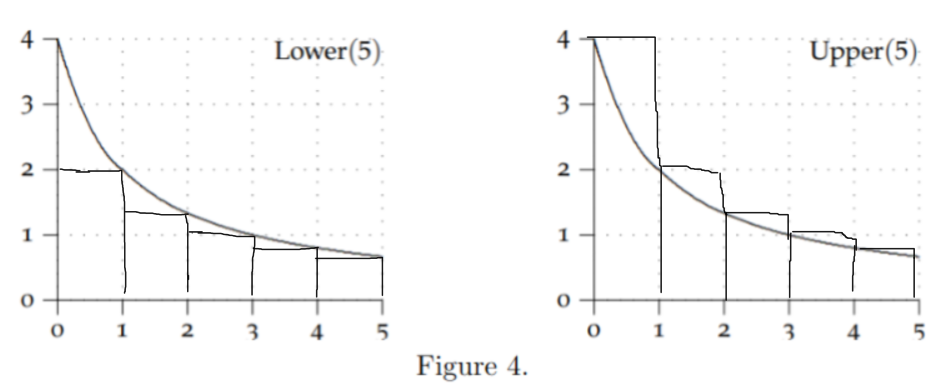
\includegraphics[scale=2]{p4.png}
\end{center}
\begin{itemize}
	\item[(a)]
		\begin{equation*}
			\mathrm{Lower}(5)\approx 2+1.3+1+0.8+0.6
			=5.7
		\end{equation*}
	\item[(b)]
		\begin{equation*}
			\mathrm{Upper}(5)\approx 4+2+1.3+1+0.8
			=9.1
		\end{equation*}
\end{itemize}

\problem{5}
\begin{center}
	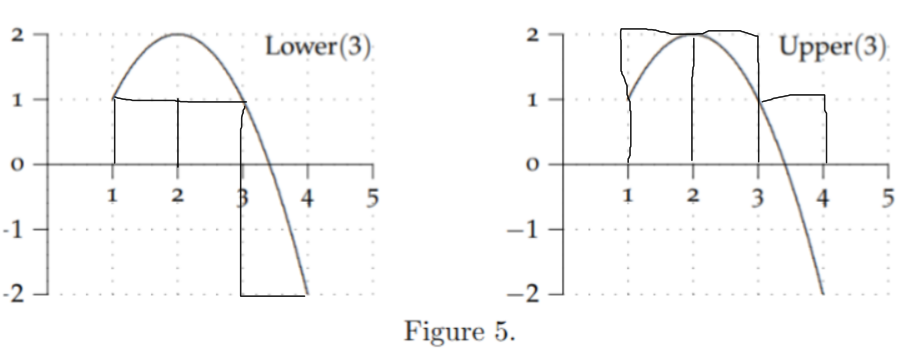
\includegraphics[scale=2]{p5.png}
\end{center}
\begin{itemize}
	\item[(a)]
		\begin{equation*}
			\mathrm{Lower}(3)=1+1+(-2)=0
		\end{equation*}
	\item[(b)]
		\begin{equation*}
			\mathrm{Upper}(3)=2+2+1=5
		\end{equation*}
\end{itemize}

\problem{6}
\begin{minipage}{0.49\linewidth}
\begin{align*}
	\Delta x&=\frac2n \\ 
	x_i&=1+\frac{2i}n \\ 
	f(x_i)&=\frac{8i}{n}+\frac{8i^2}{n^{2}} \\ 
	\sum_{i=1}^{n}f(x_i)\Delta x&=\sum_{i=1}^{n}\left(\frac{16i}{n^2}+\frac{16i^2}{n^3}\right)
\end{align*}
\end{minipage}
\begin{minipage}{0.49\linewidth}
\begin{align*}
	\Delta x&=\frac4n \\ 
	x_i&=-1+\frac{4i}n \\ 
	f(x_i)&=\frac{64i^3}{n^3} \\ 
	\sum_{i=1}^{n}f(x_i)\Delta x&=\sum_{i=1}^{n}\frac{256i^3}{n^4}
\end{align*}
\end{minipage}

\problem{7}
\begin{itemize}
	\item[(a)]
		Let $S(n)$ be the left Riemann sum with $n$ subdivisions.

		We have $\Delta x=2/n$, $x_k=1+k\Delta x=1+2k/n$.
		\begin{align*}
			S(n)&=\sum_{k=1}^{n}f(x_k)\Delta x
			=\sum_{k=1}^{n}\frac2n\left(27-\left(1+\frac{2k}{n}\right)^3\right)
			=\frac2n\sum_{k=1}^{n}27-\frac2n\sum_{k=1}^{n}\left(1+\frac{2k}{n}\right)^3 \\
			&=54-\frac2n\sum_{k=1}^{n}\left(1+\frac{2k}{n}\right)^3
			=54-\frac2n\sum_{k=1}^{n}\left[1+\frac{6k}{n}+\frac{12k^2}{n^2}+\frac{8k^3}{n^3}\right] \\
			&=54-2-\frac{12}{n^2}\sum_{k=1}^{n}k-\frac{24}{n^3}\sum_{k=1}^{n}k^2-\frac{16}{n^4}\sum_{k=1}^{n}k^3 \\
			&=52-\frac{12n(n+1)}{2n^2}-\frac{24n(n+1)(2n+1)}{6n^3}-\frac{16n^2(n+1)^2}{4n^4}\\
			&=52-\frac{6n+1}{n}-\frac{8n^2+12n+4}{n^2}-\frac{4n^2+8n+4}{n^2} \\
			\lim_{n\to\infty}S(n)&=\lim_{n\to\infty}\left[52-\frac{6n+1}{n}-\frac{8n^2+12n+4}{n^2}-\frac{4n^2+8n+4}{n^2}\right] \\
			&=\lim_{n\to\infty}\left[52-6-8-4\right]
			\tag{Trivial and left as exercise to the reader.} \\
			&=\boxed{34}
		\end{align*}
	\item[(b)]
		Let $S(n)$ be the left Riemann sum with $n$ subdivisions.

		We have $\Delta x=2/n$, $x_k=-1+k\Delta x=-1+2k/n$.
		\begin{align*}
			S(n)&=\sum_{k=1}^{n}f(x_k)\Delta x
			=\sum_{k=1}^{n}\frac2n\left(\left(-1+\frac{2k}{n}\right)^2-\left(-1+\frac{2k}{n}\right)^3\right) \\
			&=\frac2n\sum_{k=1}^{n}\left(1-\frac{4k}{n}+\frac{4k^2}{n^2}-\left(-1+\frac{6k}{n}-\frac{12k^2}{n^2}+\frac{8k^3}{n^3}\right)\right) \\
			&=\frac2n\sum_{k=1}^{n}\left(1-\frac{4k}{n}+\frac{4k^2}{n^2}+1-\frac{6k}{n}+\frac{12k^2}{n^2}-\frac{8k^3}{n^3}\right) \\
			&=\frac2n\sum_{k=1}^{n}\left(2-\frac{10k}{n}+\frac{16k^2}{n^2}-\frac{8k^3}{n^3}\right)
			=4-\frac{20}{n^2}\sum_{k=1}^{n}k+\frac{32}{n^3}\sum_{k=1}^{n}k^2-\frac{16}{n^4}\sum_{k=1}^{n}k^3 \\
			&=4-\frac{10n(n+1)}{n^2}+\frac{16n(n+1)(2n+1)}{3n^3}-\frac{4n^2(n+1)^2}{n^4} \\
			\lim_{n\to\infty}S(n)&=\lim_{n\to\infty}\left[4-\frac{10n(n+1)}{n^2}+\frac{16n(n+1)(2n+1)}{3n^3}-\frac{4n^2(n+1)^2}{n^4}\right] \\
			 &=\lim_{n\to\infty}\left[4-10+\frac{32}{3}-4\right] \tag{This statement does not warrant a proof.} \\ 
			 &=\boxed{\frac23}
		\end{align*}
\end{itemize}

\end{document}
